% (C) Anders Kofod-Petersen
\documentclass[a4paper]{book}
\usepackage{todonotes}
\presetkeys{todonotes}{color=blue!20, bordercolor=white}{}
\usepackage[english]{babel}						% Correct English hyphenation
\usepackage[utf8]{inputenc}						% Allow for non-English letters
\usepackage{graphicx}							% To include graphics
\usepackage{natbib}								% Correct citations
%\usepackage{fancyheadings}						% Nice header and footer
\usepackage[linktocpage,colorlinks]{hyperref}			% PDF hyperlink
\usepackage{geometry} 							% Better geometry
%\usepackage[center]					% For cropping documents

% B5 (uncomment to convert to B5 format)
 \geometry{b5paper}

% Author
% Fill in here, and use commands in the text. 
\newcommand{\thesisAuthor}{Olav Kåre Vatne}
\newcommand{\thesisTitle}{Segmentation in aerial images with noisy labels}
\newcommand{\thesisType}{master project}
\newcommand{\thesisDate}{spring 2015}

% PDF info
\hypersetup{pdfauthor={\thesisAuthor}}
\hypersetup{pdftitle={\thesisTitle}}
\hypersetup{pdfsubject={\thesisType}}
\hypersetup{linkcolor=black}
\hypersetup{citecolor=black}
\hypersetup{urlcolor=black}

%Fancy headings
%\pagestyle{fancy}
%\pagestyle{fancyplain}
%\renewcommand{\chaptermark}[1]{\markboth{#1}{}}
%\renewcommand{\sectionmark}[1]{\markright{#1}{}}
%\lhead[\fancyplain{}{\thepage}]{\fancyplain{}{\let\uppercase\relax\leftmark}}
%\rhead[\fancyplain{}{\let\uppercase\relax\rightmark}]{\fancyplain{}{\thepage}}
%\chead[\fancyplain{}{}]{\fancyplain{}{}}
%\lfoot[\fancyplain{}{}]{\fancyplain{}{}}
%\cfoot[\fancyplain{}{}]{\fancyplain{}{}}
%\rfoot[\fancyplain{}{}]{\fancyplain{}{}}

% Citation format
\bibliographystyle{apalike}
\bibpunct{[}{]}{;}{a}{,}{,}

\begin{document}

%Title page (This is generate automatically from the commands above)
\begin{titlepage}
\todo{New title}
\noindent {\large \textbf{\thesisAuthor}}
\vspace{2cm}

\noindent {\Huge \thesisTitle}
\vspace{2cm}

\noindent \thesisType, \thesisDate 
\vspace{2cm}

\noindent Artificial Intelligence Group\\ Department of Computer and Information Science\\ Faculty of Information Technology, Mathematics and Electrical Engineering\\

\vfill
\begin{center}

\includegraphics[width=3cm]{figs/NTNUlogo.pdf}
\end{center}
\end{titlepage}

\thispagestyle{empty}

\cleardoublepage

\frontmatter

\section*{Abstract}
\todo[inline]{Abstract- Sales pitch}
\todo[inline]{field of research, brief motivation for the work, what the research topic is, the research approach(es) applied. contributions}
\todo[inline]{Half a page of text - no lists tables or figures}

\clearpage

\section*{Preface}



\vspace{1cm}
\todo[inline]{Preface -facts}
\todo[inline]{Preface -what type of project, where it is conducted, who supervised and any acknowledgements you wish to give. }

\vfill

\hfill \thesisAuthor

\hfill Trondheim, \today

\clearpage

\tableofcontents

\listoffigures

\listoftables

\mainmatter

\chapter{Introduction}
\label{cha:Introduction}


\todo[inline]{Remember: All chapters have an introduction before sections begin, and each section begin with introduction before each subsection}
\todo[inline]{Chapters only 1 section etc subsection avoided.}
\todo[inline]{Good naming for chapter and section title. Convey meaning about contents}

\todo[inline]{clearly and concisely, avoid reptition (refer back to original discussion). All section paragraphs etc should provide new info.}
\todo[inline]{Avoid direct quotes. Only if significant}   





\section{Background and Motivation}\label{cit}
\label{sec:BackgroundAndMotivation}

\todo[inline]{Slight variation in template may be required}
\todo[inline]{Intro and background - where in the field project is situated. Driving force motivating this research. Brief}
\todo[inline]{ref to other chapters by (see code) ~\ref{T-B}}
 

\section{Goals and Research Questions}
\label{sec:Goals and Research Questions}
\todo[inline]{Research project, need question to answer. }

\begin{description}
\item[Goal] Correctly predict roads in aerial images.
\end{description}

\todo[inline]{Expand goal and clarify what is meant by goal description.}  


\begin{description}
\item[Research question 1] Handle omission and registration noise.
\end{description}
\todo[inline]{Expand, maybe}


\begin{description}
\item[Research question 2]  Curriculum learning.
\end{description}

\todo[inline]{Expand, maybe}

\section{Research Method}
\label{sec:researchMethod}

\todo[inline]{What methodology will you apply to address the goals: theoretic/analytic, model/abstraction or design/experiment? This section will describe the research methodology applied and the reason for this choice of research methodology.  }


\section{Contributions}
\label{sec:IntroContributions}
\todo[inline]{Brief main contributions (mainly in chapter~\ref{cont} }
\todo[inline]{Can be left out}

The format of this section will generally follow the following format:
{\it
Donec non turpis nec neque egestas faucibus nec id neque. Etiam consectetur, odio vitae gravida tempus, diam velit sagittis turpis, a molestie ligula tellus at nunc. Nam convallis consequat vestibulum. Proin dolor neque, dapibus a pellentesque a, commodo a nibh.}

\begin{enumerate}
\item {\it Lorem ipsum dolor sit amet, consectetur adipiscing elit.}
\item {\it Lorem ipsum dolor sit amet, consectetur adipiscing elit.}
\item {\it Lorem ipsum dolor sit amet, consectetur adipiscing elit.}
\end{enumerate}


\section{Thesis Structure}
\label{sec:thesisStructure}

\todo[inline]{Overview of what is coming in next chapter. More than explicit in chapter name, but shor and to the point}


\chapter{Background Theory and Motivation}\label{T-B}
\label{cha:TheoryAndBackground}
\todo[inline]{Intro to background theory and motivation}
{\it Lorem ipsum dolor sit amet, consectetur adipiscing elit. Nam consequat pulvinar hendrerit. Praesent sit amet elementum ipsum. Praesent id suscipit est. Maecenas gravida pretium magna non interdum. Donec augue felis, rhoncus quis laoreet sed, gravida nec nisi. Fusce iaculis fermentum elit in suscipit.}


\section{Background Theory}
\label{sec:no1}
\todo[inline]{Depth and breadth of background theory to understand project in different disciplines that your poject crosses. Help reader with theoretical basis}
\todo[inline]{Introduce terminology}
\todo[inline]{May use subsections to seperate different theory}
\todo[inline]{Intro techniques or results, reference the source}
\todo[inline]{Reference most up-to-date work in your area}
\todo[inline]{Remove how to cite and how to use figures}

The bulk of citations in the report will appear in section~\ref{cit}. However, you will often need to introduce some terminology and key citations already in this chapter. 

You can cite a paper in the following manners: 

\begin{itemize}
\item when referring to authors:\\
 \citet{authorson10:_secon_best_paper_in_world} stated something rather nice.
\item to cite indirectly: \\
 Papers should be written nicely \citep{authorson10:_secon_best_paper_in_world}\\
or\\
In \cite{authorson10:_secon_best_paper_in_world}, a less detailed template was presented.
\item To just cite the authors: \\
\citeauthor{authorson10:_secon_best_paper_in_world} wrote a nice paper.
\item Test cite: \\
\citet{Bastien-Theano-2012}
%\item Or just the year: \citeyear{authorson10:_secon_best_paper_in_world}.
%\item You can even cite specific pages: \citet[p. 3]{authorson10:_secon_best_paper_in_world}.
\end{itemize}

\vspace{0.5cm}

\noindent
{\bf Introducing figures:} \\

\begin{figure}[ht]
\begin{center}
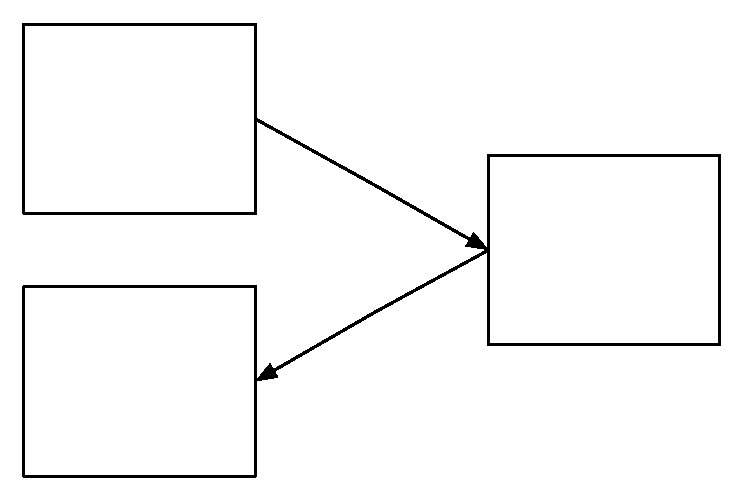
\includegraphics[width=0.5\columnwidth]{figs/figure1.pdf}
\caption[Boxes and arrows are nice]{Boxes and arrows are nice (adapted from \citet{authorson10:_secon_best_paper_in_world})}
\label{fig:BoxesAndArrowsAreNice}
\end{center}
\end{figure}
\todo[inline]{Ask for permission, figure to convey a message. Not a random figure not mentioned in the text}

\vspace{0.5cm}

\noindent
{\bf Introducing tables in the report: }\\

\begin{table}[htp]
\begin{center}
\begin{tabular}{|c|c|c|c|c|}\hline\hline
This & is & a & nice & table\\\hline
This & is & a & nice & table\\\hline\hline
\end{tabular}
\caption{Example Table}
\end{center}
\label{tab:ExampleTable}
\end{table}%
\todo[inline]{As you can see from Table \ref{tab:ExampleTable}, tables are nice. (Ref to table and draw attention to important stuff}


\section{Structured Literature Review Protocol}
\todo[inline]{As you can see from Table \ref{tab:ExampleTable}, tables are nice. Here you need to include your structured review protocol including search engine, search words, research questions  (for search, not the masters research questions), inclusion createrias and evaluation Criterias.}


\section{Motivation}
\label{sec:no2}
\todo[inline]{Application driven or methodology driven. Research focus. Other research. Why goals and questions are important to address. Present literate review. (overview of motivating elements}


\chapter{Architecture/Model}
\label{sec:architectureAndModel}
\todo[inline]{Present archtecture of model.}
\todo[inline]{No code, only figures and maybe pseudocode}


\chapter{Experiments and Results}
\label{cha:ResearchAndResults}
\todo[inline]{Introduction to experiments and results}

\section{Experimental Plan}
\label{sec:experimentalPlan}
\todo[inline]{Plan for experimental research. Include experiments and series of experiments planned.}
\todo[inline]{Planned experiments and what questions the experiements aim to answer. Connected to research questions}

\section{Experimental Setup}
\label{sec:experimentalSetup}
\todo[inline]{The experimental setup should include all data - parameters etc, that would allow a person to repeat your experiments.}

\section{Experimental Results}
\label{sec:experimentalResults}
\todo[inline]{Display results in suitable representation.}
\todo[inline]{Choose what to present}

\chapter{Evaluation and Conclusion}
\label{cha:evaluationAndConclusion}
\todo[inline]{Introduction to evaluation and conclusion}


\section{Evaluation}
\label{sec:Evaluation}
\todo[inline]{Avoid drawing grand conclusions. Only what your data can support}
\todo[inline]{Study tables graphs for unusual things that might raise questions with the reader}


\section{Discussion}
\label{sec:Discussion}
\todo[inline]{Merits and limitations}

\section{Contributions}~\label{cont}
\label{sec:Contributions}
\todo[inline]{Main contributions to the field and how significant}


\section{Future Work}
\label{sec:futureWork}
\todo[inline]{How to extend yout eotk. Directions that became obvious during work}
\todo[inline]{Possible solutions for limitations in the work conducted}


\backmatter

\addcontentsline{toc}{chapter}{Bibliography}
\bibliography{./bibtex/bibliography}

\chapter{Appendices}
\label{cha:appendices}
\listoftodos

\end{document}
